\documentclass{beamer}

\usetheme{focus}

%------------------------------------------------

\usepackage{booktabs}
\usepackage{longtable}
\usepackage{multirow}
\usepackage{colortbl}

\title{Elixir Records}

\subtitle{Programming Scalabale Systems}

\author{Jorge Sol Gonzalez \\ Paula Pousa Martinez}

\institute{jorge.sol.gonzalez@alumnos.upm.es \\ paula.pousam@alumnos.upm.es}

\date{\today}

\titlegraphic{
\includegraphics[scale=0.20]{Images/elixir.png}}

\begin{document}

%------------------------------------------------

\begin{frame}
	\maketitle
\end{frame}

%------------------------------------------------

\begin{frame}{¿What is Elixir Records?}
	\begin{block}{Objective}
    Web application to register users assistance to events.
	\end{block}
  \begin{center}
  
\includegraphics[scale=0.5]{Images/logo.png}
  \end{center}
\end{frame}

\begin{frame}{Project Architecture}
  \begin{center}
  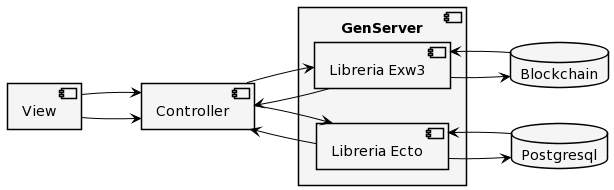
\includegraphics[scale=0.5]{Images/arquitectura.png}
  \end{center}
\end{frame}

%------------------------------------------------


\begin{frame}{Error keccakf1600}
  \begin{itemize}
    \item \textbf{ABI}: keccakf1600\_orig ~> 2.0.0 (app: keccakf1600)
    \item \textbf{Blockchain}: keccakf1600\_orig ~> 2.0.0 (app: keccakf1600)
  \end{itemize}
  \begin{center}
  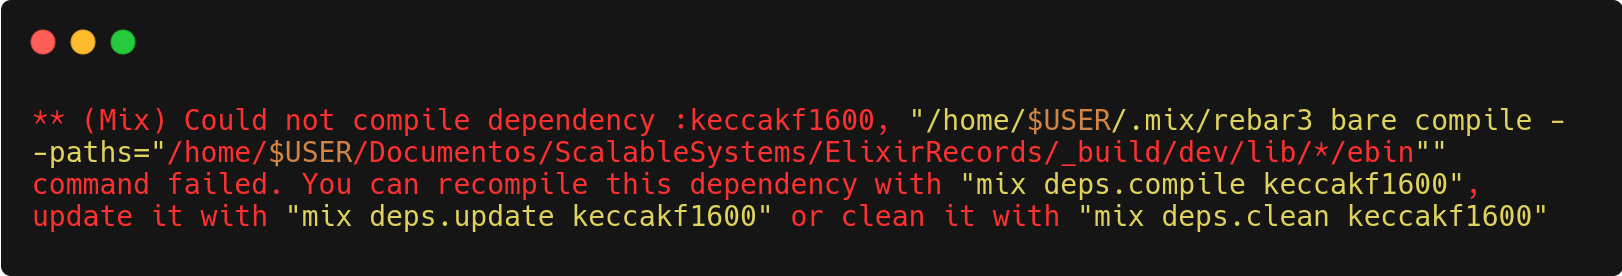
\includegraphics[scale=0.20]{Images/error.png}
  \end{center}
\end{frame}

\begin{frame}{Elixir Workers}
  \begin{center}
  
\includegraphics[scale=0.5]{Images/worker.png}
  \end{center}
\end{frame}

%------------------------------------------------

\begin{frame}{Tools}
  \begin{itemize}
    \item \textbf{Ecto}: Communication with the data base, \textit{Postgresql}.
    \item \textbf{Exw3}: Communication with the blockchain network, \textit{Ganache}.
    \item \textbf{GenServer}: Communication between the client and the different services.
    \item \textbf{Milligram}: To improve the web page \textit{style}.
  \end{itemize}
\end{frame}

\begin{frame}{Exw3 Library}
	\begin{exampleblock}{\scriptsize Advantages}
    \begin{itemize}
      \item {\footnotesize Allows basic functionalities.}
        \begin{itemize}
          \item {\footnotesize Deploys Smart Contracts.}
          \item {\footnotesize Creates new users.}
          \item {\footnotesize Interacts with Smart Contract.}
          \item {\footnotesize Sends transactions.}
        \end{itemize}
      \item {\footnotesize Easy to use.}
      \item {\footnotesize Brings all the necessary dependencies by default.}
    \end{itemize}
	\end{exampleblock}
	\begin{alertblock}{\scriptsize Disadvantages}
    \begin{itemize}
      \item {\footnotesize Lack of documentation.}
      \item {\footnotesize Some methods are implemented but doesn't seem to work.}
      \item {\footnotesize Only compatible with Ethereum networks, like Ganache.}
      \item {\footnotesize It seems impossible to recover blockchain events.}
    \end{itemize}
	\end{alertblock}
\end{frame}

\begin{frame}
  \begin{center}
  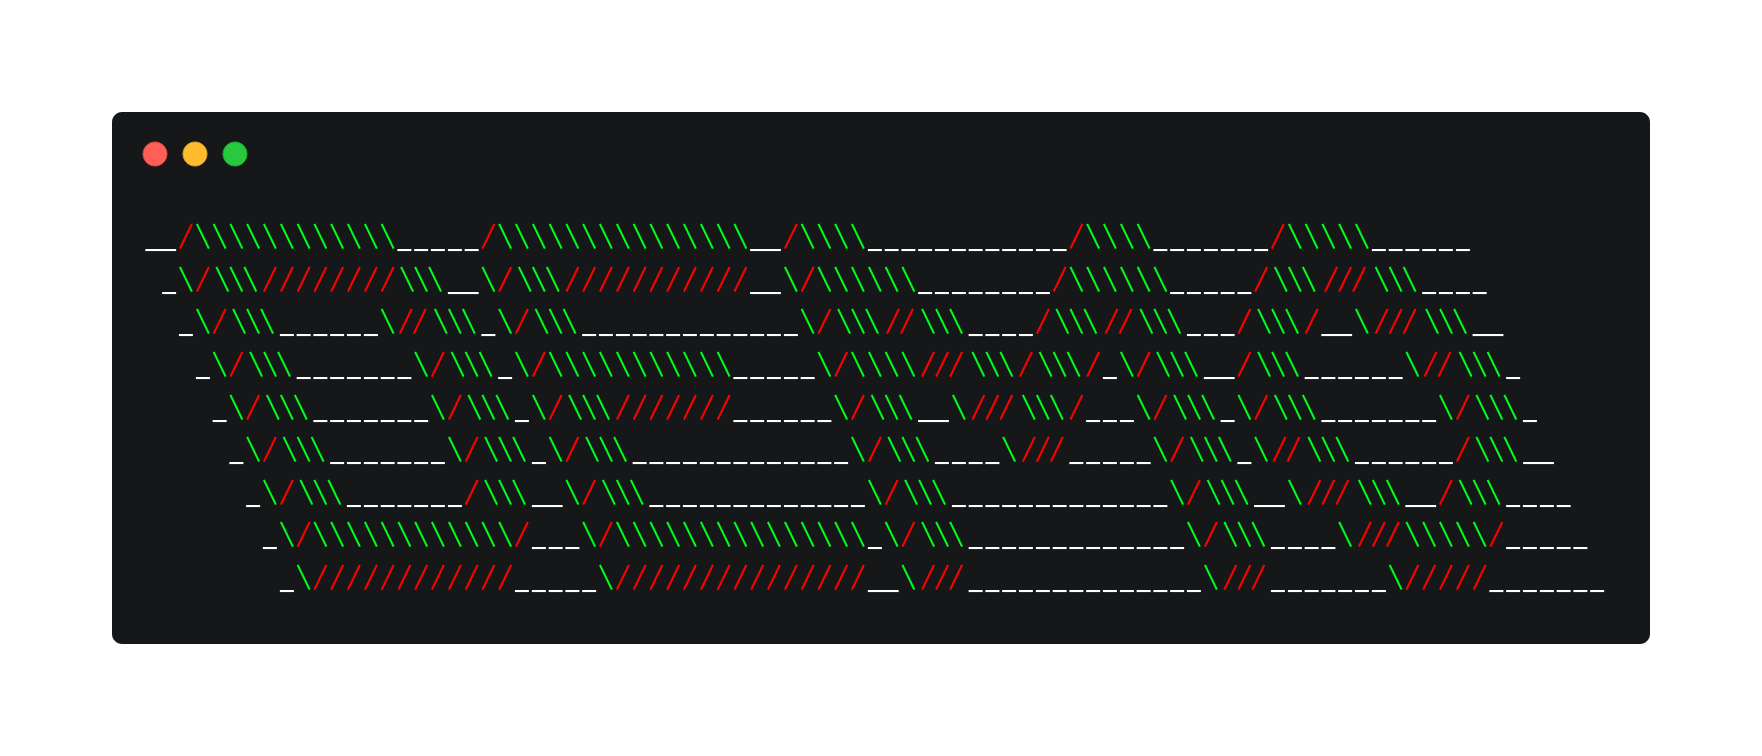
\includegraphics[scale=0.15]{Images/demo.png}
  \end{center}
\end{frame}

\end{document}
